\documentclass[a4paper,11pt,article]{memoir}

%%%%%%%%%%%%%%%%%%%%%%%%%%%%%%%%%%%%%%%%%%
% Fonts
\usepackage[T1]{fontenc}
\usepackage[utf8]{inputenc}
\usepackage[francais]{babel}
\usepackage{microtype}
\usepackage{lmodern}

\usepackage[scaled=0.95]{helvet}
\renewcommand\familydefault{\sfdefault}
\usepackage[EULERGREEK]{sansmath}\sansmath % sans-serif math w/ greeks

%%%%%%%%%%%%%%%%%%%%%%%%%%%%%%%%%%%%%%%%%%
% Page layout

\usepackage[margin=2cm]{geometry}
\pagestyle{plain}
\setlength{\parindent}{0pt}

\renewcommand*{\chaptitlefont}{\secheadstyle}% for toc, bib, and friends 
\setsecheadstyle{\Large} % default: \Large\bfseries
\setsubsecheadstyle{\large} % default: \Large\bfseries
\setsecnumdepth{subsubsection}
\settocdepth{subsubsection}
\renewcommand*{\thesection}{\arabic{section}}
\renewcommand*{\thesubsection}{\thesection.\arabic{subsection}}
\setbeforesecskip{3 ex plus 1ex minus 1ex} % default(ex): 3.5+1-.2
\setaftersecskip{2 ex plus 1ex minus 1ex} % default(ex): 2.3+.2
\setbeforeparaskip{2 ex plus 1ex minus 1ex}% default(ex): 3.25+1-.2

\setcounter{secnumdepth}{3}

\renewcommand\title[1]{{\LARGE\fontfamily{pag}\selectfont #1}\par\bigskip}

%%%%%%%%%%%%%%%%%%%%%%%%%%%%%%%%%%%%%%%%%%%
% Utilities


% \usepackage{minted} % syntax coloring % If you don't have the
% 'minted' package, just turn all listings to verbatim :-)

\usepackage{boxedminipage}

\newenvironment{reponse}{
\begin{center}
  \begin{boxedminipage}{0.9\linewidth}\underline{Réponse}~:~
}{
  \end{boxedminipage}
\end{center}
}

\usepackage{graphicx}


%%%%%%%%%%%%%%%%%%%%%%%%%%%%%%%%%%%%%%%%%%%
% Document body

\begin{document}

\includegraphics[height=2cm]{fig/insa.pdf}
%
\hfill
%
{\fontfamily{pag}\selectfont Département IF / Architecture Matérielle}

\bigskip

\title{TP2: Développement Croisé}

\bigskip
\noindent\par\parbox{.48\textwidth}{Nom : Bertron} \parbox{.48\textwidth}{Prénom : Aurélien}
\bigskip
\noindent\par\parbox{.48\textwidth}{Nom : Losbar} \parbox{.48\textwidth}{Prénom : Thomas}
\bigskip
\noindent\par\parbox{.2\textwidth}{Groupe : 2} \parbox{.2\textwidth}{Binôme : B3229}

\bigskip

\paragraph{Question 1 ---}  La fonction lcd_init() écrit dans les registres LCDACTL, LCDAPCTL (0 et 1) et LCDMEM (1 à 20).

\paragraph{Question 2 ---}  

\paragraph{Question 3 ---}  D'après MSP430.pdf[750], tous les registres font 8 bits. D'après datasheet.pdf[16], les registres 8 bits de périphériques sont situés entre les adresses 0FFh et 010h.

\paragraph{Question 4 ---}  Les plages d'adresses sont spécifiées à la même adresse :
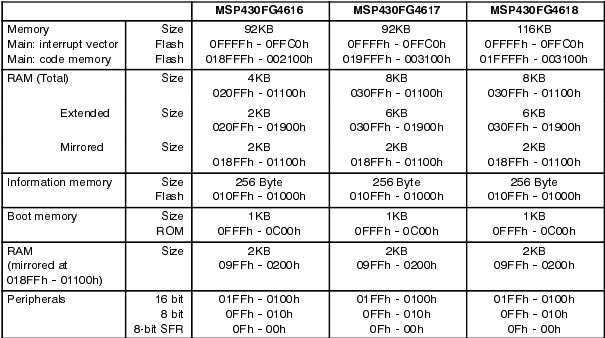
\includegraphics[height=4cm]{fig/plagesAdressage.pdf}

\paragraph{Question 5 ---}  Dans Compiler.pdf[207], on peut voir qu'en C, l'opérateur @ permet de définir l'adresse à laquelle est stockée une variable. Ces deux lignes sont des déclarations de macros qui permettent de définir une variable à une adresse donnée. La seule différence est la taille de la zone mémoire : 16 bits pour DEFW, 8 bits pour DEFC.

\paragraph{Question 6 ---}  Trouvé dans MSP430.pdf[750/736] : on voit que {f_LCD = 2 \times mux \times f_frame}, on cherche f_frame. On indique dans le code que l'on divise ACLK par 512 (bits 5,6 et 7 de LCDACTL à 1). f_LCD est donc égal à 32768 / 512 = 75,71 Hz. Donc f_frame = f_LCD / (2 * 4) = 9,46Hz, car mux = 4.

\paragraph{Question 7 ---}  Il nous faut changer les 3 derniers bits de LCDACTL. C'est à ça que sert la ligne 21 "(n<<5)", c'est à dire écrire n à partir du 5ème bit dans LCDACTL. Au lien de diviser ACLK par 512, on choisit de diviser par 128, ce qui donne une valeur pour f_frame de 32 Hz. L'écran ne scintille plus.

\paragraph{Question 8 ---}  A la ligne LCDMEM[j] = 0xFF, on change 0xFF par 0 pour éteindre tous les segments.

\paragraph{Question 9 ---}  Le boîtier de l'écran possède 26 broches. LCD.pdf[3] nous montre qu'il y a 4 broches communes et 22 segments pins.

\paragraph{Question 10 ---}  22 * 4 = 88, il y a donc en tout 88 segments sur l'écran.

\paragraph{Question 11 ---}  Selon LCD.pdf[3], Dollar correspond à COM0 (P18) et à P26.

\paragraph{Question 12 ---}  Selon CPU.pdf[19], la pin 26 de l'écran est reliée à la pin 37 du MSP430. COM0 est reliée à la pin 52 du MSP430.

\end{document}
